\documentclass[border=4pt]{standalone}

\usepackage[T1]{fontenc}
\usepackage[utf8]{inputenc}
\usepackage{amsmath}
\usepackage{xcolor}
\usepackage{tikz}
\usetikzlibrary{positioning, fit, calc, arrows.meta, backgrounds}

\pgfdeclarelayer{background}
\pgfsetlayers{background,main}

% ── palette (matches unet_entity_cbam_deep / training_pipeline) ──────
\definecolor{inputcol}{RGB}{239,159,39}    % orange : inputs
\definecolor{enginecol}{RGB}{133,183,235}  % blue   : execution engine
\definecolor{servercol}{RGB}{175,169,236}  % purple : RL agents
\definecolor{intercol}{RGB}{160,160,150}   % gray   : raw output
\definecolor{analysiscol}{RGB}{93,202,165} % teal   : analysis
\definecolor{resultcol}{RGB}{120,190,90}   % green  : result

\begin{document}

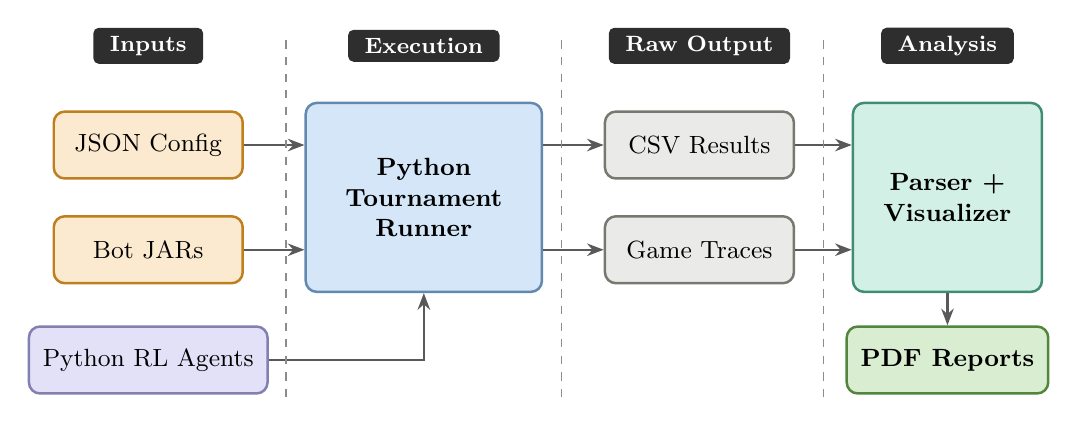
\begin{tikzpicture}[
    scale=0.7,
    >={Stealth[length=6pt]},
    %% ── Base node style ──
    box/.style={
        rectangle, draw, line width=0.9pt, rounded corners=4pt,
        align=center, font=\small, inner sep=5pt
    },
    %% ── Specialized styles (saturated fills + strong colored borders) ──
    input/.style={box, fill=inputcol!22, draw=inputcol!80!black,
        minimum width=2.4cm, minimum height=0.85cm},
    engine/.style={box, fill=enginecol!35, draw=enginecol!75!black,
        minimum width=3cm, minimum height=2.4cm, font=\small\bfseries},
    server/.style={box, fill=servercol!35, draw=servercol!75!black,
        minimum width=2.4cm, minimum height=0.85cm},
    intermediate/.style={box, fill=intercol!22, draw=intercol!75!black,
        minimum width=2.4cm, minimum height=0.85cm},
    analysis/.style={box, fill=analysiscol!28, draw=analysiscol!70!black,
        minimum width=2.4cm, minimum height=2.4cm, font=\small\bfseries},
    result/.style={box, fill=resultcol!28, draw=resultcol!70!black,
        minimum width=2.4cm, minimum height=0.85cm, font=\small\bfseries},
    %% ── Arrow / label styles ──
    flow/.style={->, line width=0.9pt, color=black!65},
    %% black "pill" phase badges (signature element) ──
    phasepill/.style={fill=black!82, text=white, rounded corners=2pt,
        inner xsep=6pt, inner ysep=3pt, font=\footnotesize\scshape\bfseries},
]

% ── Phase labels (black pills) ──
\node[phasepill] at (0,    2.5) {Inputs};
\node[phasepill] at (5,    2.5) {Execution};
\node[phasepill] at (10,   2.5) {Raw Output};
\node[phasepill] at (14.5, 2.5) {Analysis};

% ── Column 1 · Inputs ──
\node[input]  (config) at (0,  0.7)  {JSON Config};
\node[input]  (jars)   at (0, -1.2)  {Bot JARs};
\node[server] (socket) at (0, -3.2)  {Python RL Agents};

% ── Column 2 · Execution ──
\node[engine] (engine) at (5, -0.25) {Python\\Tournament\\Runner};

% ── Column 3 · Raw Output ──
\node[intermediate] (csv)    at (10,  0.7) {CSV Results};
\node[intermediate] (traces) at (10, -1.2) {Game Traces};

% ── Column 4 · Analysis ──
\node[analysis] (parser) at (14.5, -0.25) {Parser +\\Visualizer};
\node[result]   (viz)    at (14.5, -3.2)  {PDF Reports};

% Row A  (y = 0.7)
\draw[flow] (config.east)             -- (engine.west |- config.east);
\draw[flow] (engine.east |- csv.west) -- (csv.west);
\draw[flow] (csv.east)                -- (parser.west |- csv.east);

% Row B  (y = -1.2)
\draw[flow] (jars.east)                  -- (engine.west |- jars.east);
\draw[flow] (engine.east |- traces.west) -- (traces.west);
\draw[flow] (traces.east)                -- (parser.west |- traces.east);

% L-shape: Socket → Engine  (horizontal then vertical)
\draw[flow] (socket.east) -| (engine.south);

% Vertical: Parser → PDF Reports
\draw[flow] (parser.south) -- (viz.north);

% ── Phase separators (midpoints between columns) ──
\draw[dashed, color=black!45] (2.5,  2.6) -- (2.5,  -4.0);
\draw[dashed, color=black!45] (7.5,  2.6) -- (7.5,  -4.0);
\draw[dashed, color=black!45] (12.25, 2.6) -- (12.25, -4.0);

\end{tikzpicture}

\end{document}
